\section{Technische Dokumentation}
\subsection{Dokumentation der Storys}

\subsubsection{Der Benutzer möchte ein Fenster}

\begin{enumerate}
 \item Das Fenster ist sichtbar
 \item Das Fenster hat eine festgelegte größe
 \item Das Fenster kann verschoben werden
\end{enumerate}

\textbf{Storypoints:} 2 \\
\textbf{Bearbeitet von:} Fabian Zeller \\
\\
\textbf{Beschreibung:} Ein einfaches Fenster ohne Inhalt war nicht schwer zu verwirklichen. Das Fenster ist ein einfaches JPanel.


\subsubsection{Der Benutzer möchte 3 Sektionen in dem Fenster}


\begin{enumerate}
 \item Die Sektionen sollen beschriftet sein
 \item Sektionen untereinander"
\end{enumerate}

\textbf{Storypoints:} 2 \\
\textbf{Bearbeitet von:} Fabian Zeller \\
\\
\textbf{Beschreibung:} Das ursprüngliche JPanel wurde zu der contentpane. Drei weitere Panels wurden untereinander angeordnet hinzugefügt.


\subsubsection{Der Benutzer möchte, dass in der unteren Sektion Klaviertasten angezeigt werden}

\begin{enumerate}
 \item Die Tasten haben 2 Farben (schwarz/weiß)
 \item Die Tasten können angeklickt werden
 \item Die Tasten sind wie auf einem Klavier angeordnet
\end{enumerate}

\textbf{Storypoints:} 5 \\
\textbf{Bearbeitet von:} Fabian Zeller \\
\\
\textbf{Beschreibung:} Die Klaviertasten bestehen aus jeweils      bis    kleineren Toggle Buttons. Dies wurden so konfiguriert dass sie wie Klaviertasten aussehen. 


\subsubsection{Der Benutzer möchte mittels Tasten (Tastatur) einen Klavierton abspielen}

\begin{enumerate}
 \item Die Tasten spielen jeweils genanu einen Ton wenn sie geklickt werden
 \item Die Tasten können einen Ton halten
\end{enumerate}

\textbf{Storypoints:} 5 \\
\textbf{Bearbeitet von:} Emanuel Hubenschmid \\
\\
\textbf{Beschreibung:} Zu Begin versuchten wir dies über eine Synthesizer-Klasse der 
Javabibliothek. Dies erwies sich allerdings als äußerst umständlich. Deswegen entschlossen wir uns 
die Samples selber zusammen zu stellen und diese als Clips aufzurufen.


\subsubsection{Der Programmierer arbeitet sich in Git-Hub ein}

\begin{enumerate}
 \item Das Git-Hub Repository kann von allen Programmierern benutzt werden
\end{enumerate}

\textbf{Storypoints:} 3 \\
\textbf{Bearbeitet von:} Fabian Zeller, Emanuel Hubenschmid \\
\\
\textbf{Beschreibung:} Um die Zusammenarbeit zu erleichtern verwendeten wir GitHub zur Verwaltung 
unseres Projektes (Siehe \textbf{\ref{sssec:GitHub} GitHub})


\subsubsection{Der Programmierer arbeitet sich in Javadocs ein}

\begin{enumerate}
 \item Die Javadoc-Seite soll alle wichtigen Informationen zu dem Programmquellcode enthalten
 \item Die Javadoc-Seite soll in der Dokumentation verlinkt werden
\end{enumerate}

\textbf{Storypoints:} 3 \\
\textbf{Bearbeitet von:} Fabian Zeller, Emanuel Hubenschmid \\
\\
\textbf{Beschreibung:} Wir entschieden uns unseren Quelltext mittels Javadocs auszukemmentieren. 
Dies bot uns die möglichkeit den überblick zu behalten und dem jeweils anderem eine einfache 
möglichkeit zu bieten den Quelltext besser zu verstehen.


\subsubsection{Der Benutzer möchte, dass die gespielte Taste hervorgehoben wird}

\begin{enumerate}
 \item Wenn eine Taste auf der Tastatur betätigt wird, färbt sich die entsprechende Taste auf dem 
Bildschirm
\end{enumerate}

\textbf{Storypoints:} 5 \\
\textbf{Bearbeitet von:} Fabian Zeller \\
\\
\textbf{Beschreibung:} Der Taste auf der Tastatur wird eine Gruppe von Toggle Buttons zugewiesen, die dann wie eine taste von einem Klavier aussehen. Diese werden dann betätigt.


\subsubsection{Der Benutzer möchte voreingestellte Samples auswählen können}

\begin{enumerate}
 \item Die Sample sollen die Tasten mit unterschiedlichen Tönen belegen
 \item Die voreingestellten Samples sollen Klaviertöne und Schlagzeugtöne 
abspielen
\end{enumerate}

\textbf{Storypoints:} 5 \\
\textbf{Bearbeitet von:} Emanuel Hubenschmid \\
\\
\textbf{Beschreibung:} Das Programm sollte eine möglichkeit bieten, direkt etwas spielen zu können. 
Da die Java Sound API nur .wav Dateien mit 8 oder 16 Bit, mussten wir auch solche Sounddateien als 
Samples verwenden. Die Samples können über Radiobutton ausgewählt werden.


\subsubsection{Der Benutzer möchte mehrere Töne gleichzeitig spielen können}

\begin{enumerate}
 \item Die Töne sollen gleichzeitig abgespielt werden können
 \item Die Töne sollen nicht durch andere Töne unterbrochen werden
 \item Die Töne, die gleichzeitig angespielt wurden, sollen auch gleichzeitig abgespielt werden
 \item Die  anzahl der Töne die gleichzeitig gespielt werden können ist auf 3 beschränkt
\end{enumerate}

\textbf{Storypoints:} 5 \\
\textbf{Bearbeitet von:} Emanuel Hubenschmid \\
\\
\textbf{Beschreibung:} Damit Töne gleichzeitig abgespielt werden können müssen diese über 
einen Thread in einem Vektor erzeugt und gestartet werden. Der Key Buffer kann jedoch nicht 
mehr als 3 Tasten gleichzeitig erfassen.


\subsubsection{Der Benutzer möchte, dass in der oberen Sektion Notenlinien angezeigt werden}

\begin{enumerate}
 \item Die Notenlinien bestehen aus fünf Linien
 \item Die Notenlinien beginnen mit einem Notenschlüssel
\end{enumerate}

\textbf{Storypoints:} 5 \\
\textbf{Bearbeitet von:} Fabian Zeller \\
\\
\textbf{Beschreibung:} Mehrere Images von leeren Noten werden der oberen Sektion hinzugefügt.


\subsubsection{Der Benutzer möchte Notenlblätter, auf denen Noten angezeigt und abgespeichert werden}

\begin{enumerate}
 \item 
 \item 
 
\end{enumerate}

\textbf{Storypoints:} 5 \\
\textbf{Bearbeitet von:} Emanuel Hubenschid \\
\\
\textbf{Beschreibung:} 


\subsubsection{Der Benutzer möchte das gespielte Töne als Note angezeigt werden}

\begin{enumerate}
 \item Noten laufen die Notenlinie entlang
 \item Vorzeichen bei bestimmten Noten
\end{enumerate}

\textbf{Storypoints:} 8 \\
\textbf{Bearbeitet von:} Fabian Zeller \\
\\
\textbf{Beschreibung:} Ein leeres Bild wird durch das Bild der entsprechend gespielten Note ersetzt.


\subsubsection{Der Benutzer möchte das gespeicherte Notenlinien in einem externen Fenster aufgerufen 
werden können}

\begin{enumerate}
 \item Die Notenlinien  werden in einem externen Fenster geöffnet
\end{enumerate}

\textbf{Storypoints:} 5 \\
\textbf{Bearbeitet von:} Emanuel Hubenschmid \\
\\
\textbf{Beschreibung:} Wird eine Datei abgespielt öffnet sich ein seperates Fenster, in welchem der 
Player die gerade abgespielte Note abbildet.


\subsubsection{Der Benutzer möchte gespeicherte Notenlinien abspielen}

\begin{enumerate}
 \item Die Notenlinien  können abgespielt, pausiert und gestoppt werden
\end{enumerate}

\textbf{Storypoints:} 8 \\
\textbf{Bearbeitet von:} Emanuel Hubenschmid \\
\\
\textbf{Beschreibung:} Die gespeicherten Noten werden aus einer Textdatei ausgelesen und 
abgespielt. Ein Button kann diese nun pausieren. Wird das Fenster geschlossen, wird auch die Datei 
gestoppt.


\subsubsection{Der Benutzer möchte Noten, die auf den Notenlinien angezeigt und abgespeichert 
werden}

\begin{enumerate}
 \item Die Noten, die gespielt wurden, sollen auf den richtigen Notenlinien angezeigt werden
 \item Die Noten sollen die Tonhöhe speichern
\end{enumerate}

\textbf{Storypoints:} 8 \\
\textbf{Bearbeitet von:} Fabian Zeller, Emanuel Hubenschmid \\
\\
\textbf{Beschreibung:} Wird während der Aufnahme eine Taste gedrückt wird diese in ein Textdokument 
geschrieben.


\subsubsection{Der Entwickler möchte eine Latex Dokumentation}

\begin{enumerate}
 \item Deckblatt
 \item Inhaltsverzeichniss
 \item Link auf Javadocs
 \item Quellen
\end{enumerate}

\textbf{Storypoints:} 5 \\
\textbf{Bearbeitet von:} Fabian Zeller, Emanuel Hubenschmid \\
\\
\textbf{Beschreibung:} Ich arbeite daran.


\subsubsection{Der Benutzer möchte ein ToolBar-Menü}

\begin{enumerate}
 \item Die ToolBar enthält ein Hilfe-Menü
 \item Die ToolBar enthält ein Projekt Öffnen-Menü
 \item Die ToolBar enthält ein Neues Projekt-Menü
\end{enumerate}

\textbf{Storypoints:} 3 \\
\textbf{Bearbeitet von:} Fabian Zeller, Emanuel Hubenschmid \\
\\
\textbf{Beschreibung:} Wir entschieden uns dazu keine Untermenüs zu verwenden, da bei einer so 
geringen anzahl an Optionen, dies viel umständlicher für den Benutzer währe.


\subsubsection{Der Benutzer möchte, dass in der Mittleren Sektion Buttons zur Steuerung angezeigt 
werden}

\begin{enumerate}
 \item Samples können über Radiobutton ausgewählt werden
\end{enumerate}

\textbf{Storypoints:} 3 \\
\textbf{Bearbeitet von:} Emanuel Hubenschmid \\
\\
\textbf{Beschreibung:} Ürsprünglich waren die Button zur Aufnahme und Wiedergabe ebenfalls in 
diesem Bereich geplant. Diese sind jedoch nun Projektgebunden und deswegen in dem Projektfenster. 
Es finden sich hier nurnoch die Radiobutton zur Auswahl der Sample.


\subsubsection{Der Benutzer möchte mit der Leertaste alle geöffneten Aufnahmen abspielen}

\begin{enumerate}
 \item Die Leertaste startet oder Stoppt alle geöffneten Aufnahmen
\end{enumerate}

\textbf{Storypoints:} 8 \\
\textbf{Bearbeitet von:} Emanuel Hubenschmid \\
\\
\textbf{Beschreibung:} Damit alle Aufnahmen gleichzeitig abgespielt werden können und als ``ganzes 
Lied'' gehört werden können. Ermöglicht es die Leertaste alle geöffneten Aufnahmen gleichzeitig 
abzuspielen.


\subsubsection{Der Benutzer möchte eingene Samples benutzen können}

\begin{enumerate}
 \item Die Samples sollen in eine Bibliothek geladen werden können
 \item Die Samples sollen vom Benutzer ausgewählt und abgespielt werden können
\end{enumerate}

\textbf{Storypoints:} 5 \\
\textbf{Bearbeitet von:} Emanuel Hubenschmid \\
\\
\textbf{Beschreibung:} Am einfachsten und übersichtlichsten erwies es sich, eigene Samples nur mit 
einem Projekt verwenden zu können. Diese sind dabei immer in dem Projekt-Ortner unter Samples in 
einem Ortner abzuspeichern.


\subsubsection{Der Benutzer möchte einen Projektordner erzeugen können}

\begin{enumerate}
 \item Der Projektordner enthält eine Sample- und einen Aufnahme-Ordner
\end{enumerate}

\textbf{Storypoints:} 8 \\
\textbf{Bearbeitet von:} Emanuel Hubenschmid \\
\\
\textbf{Beschreibung:} Wird ein neues Projekt erstellt speichert dies nur den Ordnerpfad in dem 
sich die Samples und Aufnahmen befinden.


\subsubsection{Der Benutzer möchte das die Note einer Taste auf der Taste angezeigt wird}

\begin{enumerate}
 \item Sichtbare Note auf den Tasten
\end{enumerate}

\textbf{Storypoints:} 5 \\
\textbf{Bearbeitet von:} Fabian Zeller \\
\\
\textbf{Beschreibung:} Eine Glasspane mit entsprechender Beschriftung wurde über die GUI gelegt.


\subsubsection{Der Benutzer möchte die Samples wechseln}

\begin{enumerate}
 \item Die Samples sollen mittels RadioButton ausgewählt werden können,
 \item Die RadioButton sollen für jede Taste das gleiche Sample auswählen
 \item Die Samples sollen mit Tasten gewächselt werden können"
\end{enumerate}

\textbf{Storypoints:} 5 \\
\textbf{Bearbeitet von:} Emanuel Hubenschmid \\
\\
\textbf{Beschreibung:} Ist ein Radiobutton ausgewählt wird der Ordnerpfad 
des jeweiligen Samples benutzt um den Clip zu starten.


\newpage

\subsection{Klassendiagramme}

{\centering
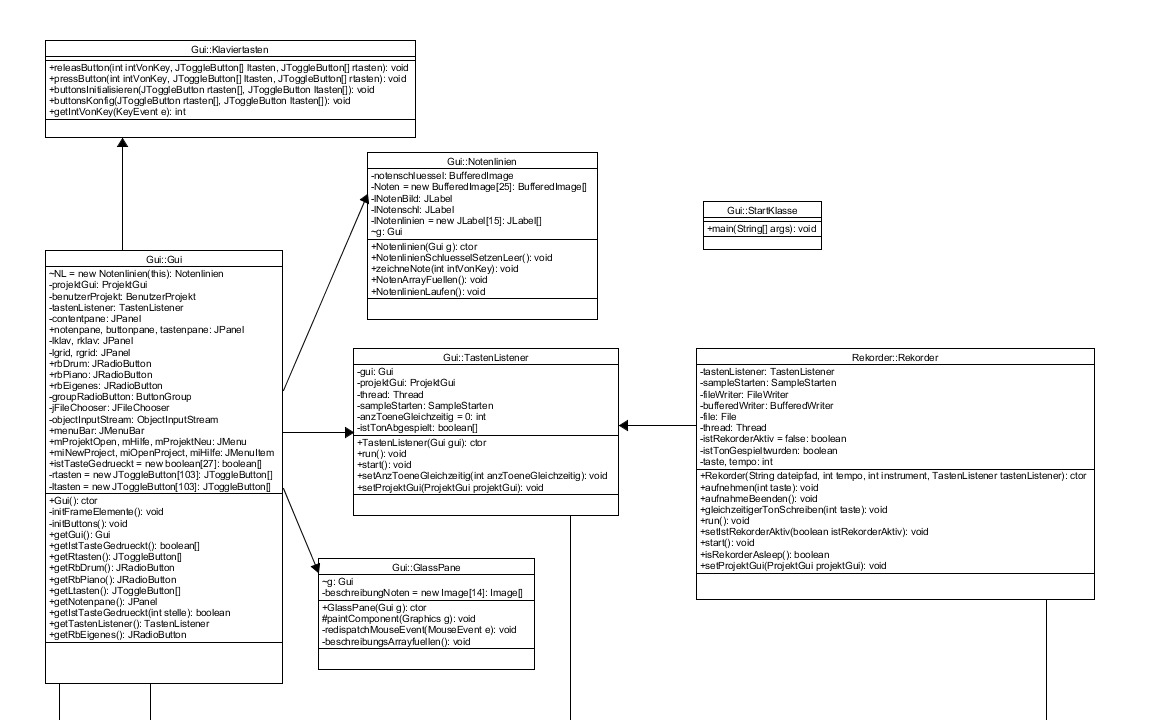
\includegraphics[scale=0.5]{Bilder/GUIKlassendia/TeilOben.PNG} 

\medskip
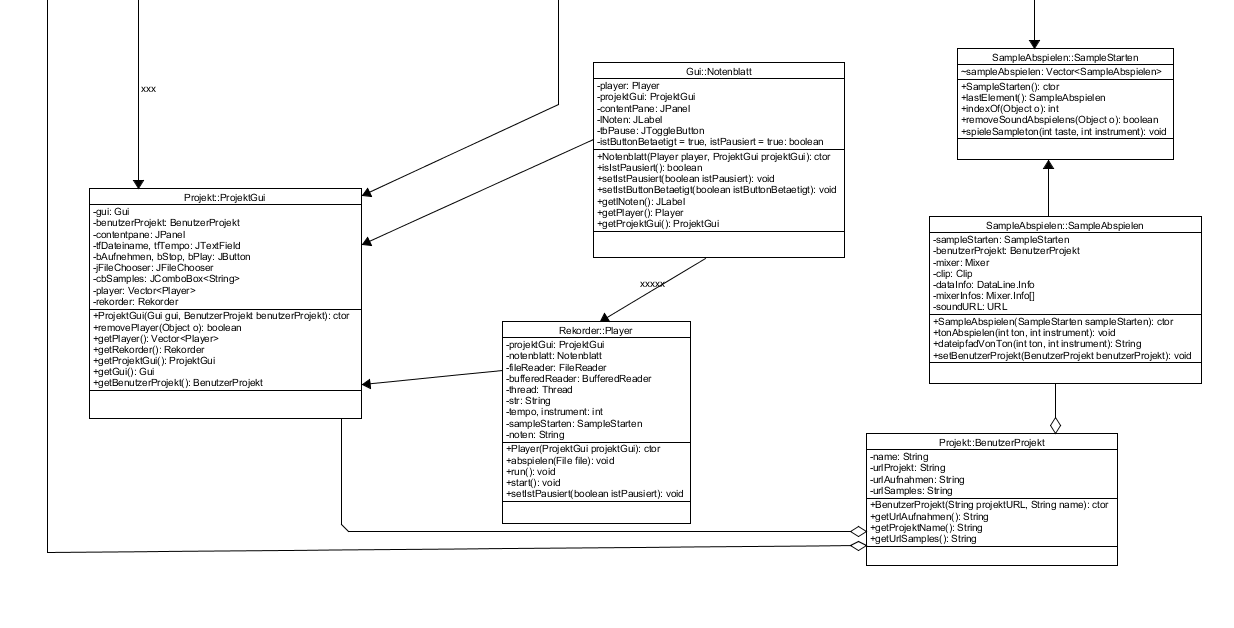
\includegraphics[scale=0.5]{Bilder/GUIKlassendia/TeilUnten.PNG} 

}

\newpage

\newpage

\subsection{Sequenzdiagramme}


\begin{figure}[h]
 \centering
 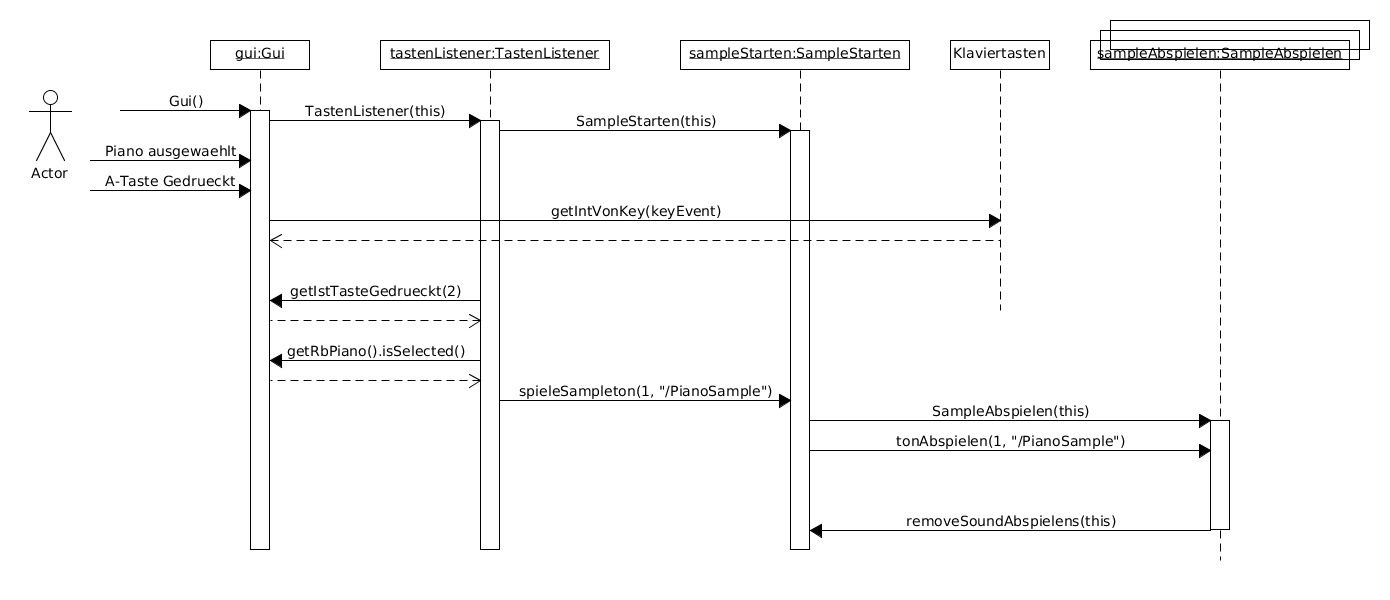
\includegraphics[width=1\textwidth]{./Bilder/Klaviertaste_Gedrueckt.png}
 \caption{Sequenzdiagramm für das Abspielen eines Tones}
\end{figure}

fehler verbessern

\paragraph{Beschreibung:} In diesem Szenario will der Benutzer das untere Cis des Piano Samples 
abspielen. Als erstes startet dieser das Programm und erzeugt dadurch ein Gui-Objekt. Als nächstes 
wählt er das Piano Sample über die Radiobutton aus (Piano ist zu Begin ausgewählt). Drückt der 
Benutzer nun die A-Taste wird der Ton abgespielt.\\
Damit der Ton abgespielt werden kann benötigt das Programm ein TastenListener-Objekt welches 
ständig abprüft, ob eine der, mit Tönen belegten Tasten, gedrückt wurde. Dieses Objekt wird im 
Konstruktor der Gui erzeugt.\\
Um nun einen Ton starten zu können, wird ein SampleStarten-Objekt benötigt. Dies wird im 
Konstruktor des TastenListener-Objektes erzeugt.\\
Wird nun die A-Taste gedrückt, sucht die Methode getIntVonKey(KeyEvent keyEvent) in der Klasse 
Klaviertasten, den der Taste zugewiesene Integer-Wert (die A-Taste hat den Wert 1). Mit diesem Wert 
kann man nun das Array istTasteGedrückt an der stelle 2 auf true setzten.\\
Der TastenListener prüft dabei Ständig ab welche Tasten gedrückt wurde. Wurde eine Taste gedrückt 
frägt er noch das dabei ausgewählte Sample ab.\\
Diese Informationen schickt der TastenListener dann zu dem SampleStarten-Objekt. Welches 
wiederum, in einem Vektor, ein SampleAbspielen-Objekt erzeugt und anschließend über die Methode 
tonAbspielen den Ton abspielt.\\
Sobald der Ton abgespielt wurde löscht sich das SampleAbspielen-Objekt wieder aus dem Array.
Wie der Ton in dem SampleAbspielen-Objekt funktioniert können sie der \textbf{Abbildung 
\ref{fig:tonAbspielen}} entnehmen.


\newpage

\begin{figure}[h]
 \centering
 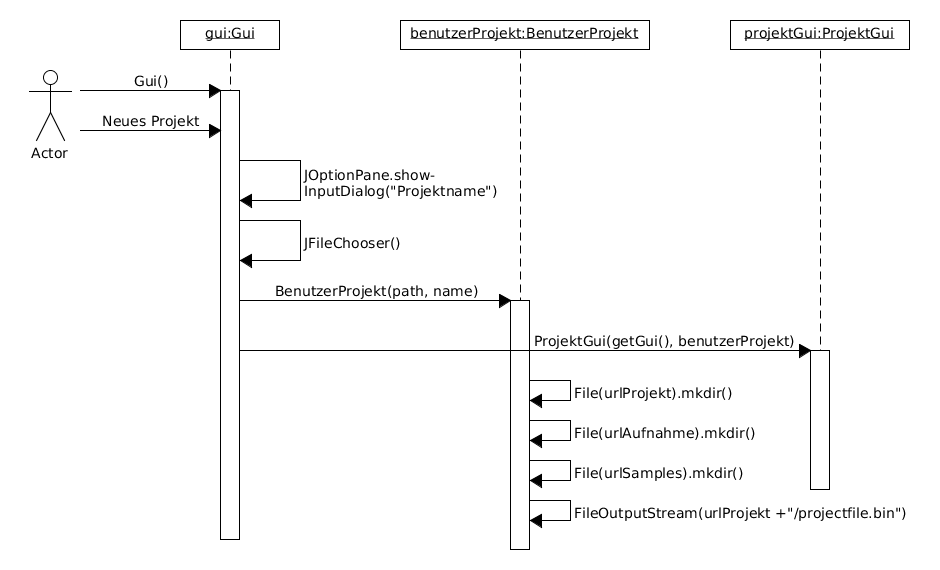
\includegraphics[width=1\textwidth]{./Bilder/Neues_Projekt.png}
 \caption{Sequenzdiagramm für erstellen eines neuen Projektes} 
\end{figure}

\paragraph{Beschreibung:} In diesem Szenario will der Benutzer ein neues Projekt erstellen. Nach 
dem Starten des Programmes und erzeugen eines Gui-Pbjektes klickt der Benutzer auf das Menü ``Neues 
Projekt'' in der ToolBar. Als nächstes gibt dieser den Namen des Projektes in einem Dialog ein und 
wählt anschließend den Dateipfad über einen FileChooser aus. Mit diesen Informationen kann nun ein 
BenutzerProjekt-Objekt erzeugt werden. Der Konstruktor der BenutzerProjekt-Klasse erzeugt dann 
einen Projekt-Ordner und in diesem ein Aufnahme-Ordner, Samples-Ordner und eine projectfile.bin 
datei. mit dem BenutzerProjekt-Objekt kann nun die ProjektGui gestartet werden.\\



\newpage

\subsection{Struktogramme}


\begin{figure}[h]
 \centering
 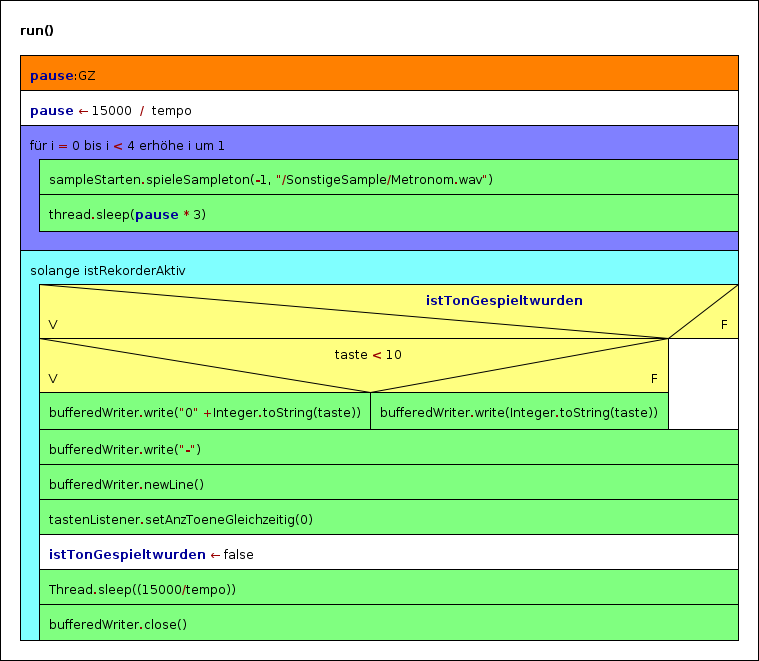
\includegraphics[width=1\textwidth]{./Bilder/Ton_Aufnehmen.png}
 \caption{Struktogramm für das Aufnehmen eines Tones}
\end{figure}

\paragraph{Beschreibung:} Am Anfang der run()-Methode wird die Zeit für die Pause zwischen zwei 
16tel berechnet. Anschließend spielt die Methode 4 Metronomschläge in 4tel abständen ab. Wird kein 
Ton abgespielt, schreibt die Methode einen Bindestrich in die Aktuelle Zeile des Textdokumentes und 
wartet eine 16tel-Pause.\\
Wird ein Ton gespielt, schreibt die Methode dessen ID-Nummer in das Textdokument (bei einstelligen 
Zahlen eine Null voran gestellt werde).\\



\newpage

\begin{figure}[h]
 \centering
 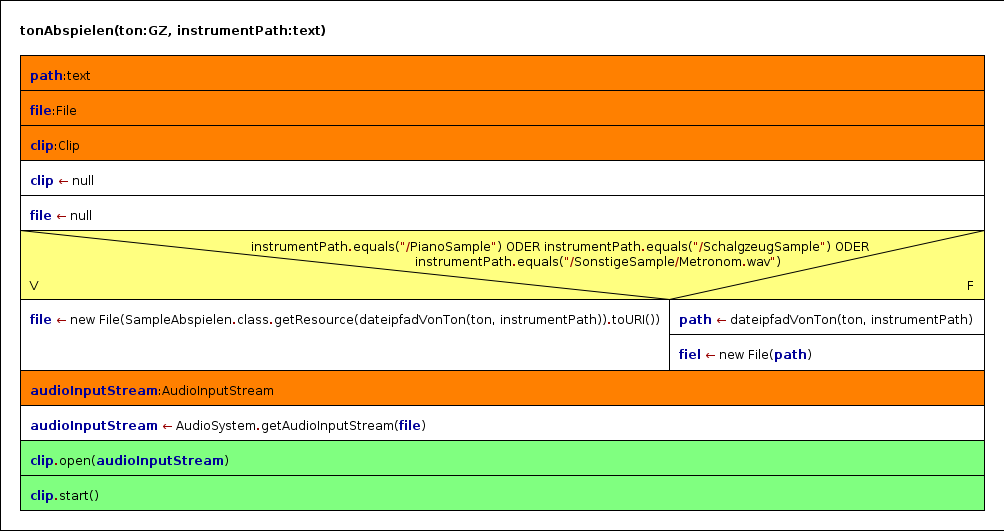
\includegraphics[width=1\textwidth]{./Bilder/tonAbspielen.png}
 \caption{Struktogramm für das Abspielen eines Tones} \label{fig:tonAbspielen}
\end{figure}

\paragraph{Beschreibung:} In dieser Methode wird ein Clip erzeugt und gestartet. Allerdings müssen 
Dateien aus dem Javaprojekt-Ordner anderst geöffnet werden als Dateien die auserhalb des 
Javaprojekts.



\subsection{JavaDocs}
Der komplette Quelltext wurde mittels Javadocs auskommentiert. Hier kann nachgelesen werden, welche 
funktion die einzelnen Methoden erfüllen, sowie ihre Übergabe- und Rückgabeparameter, bzw. 
Exeptions  eingesehen werden.\\
Die komplette Javadocs Dokumentation kann hier geöffnet werden:\\
\url{./JavaDocs/index.html}



